It begins! Today will be entirely tutorials---I arrived just in time for the second half of the PAC-Bayes tutorial. 

\subsection{Tutorial: PAC-Bayes Theory (Part II)}

{\bf Part I Recap:}~\citet{shawe1997pac} carried out PAC~\cite{valiant1984theory} analysis of Bayesian estimators (also see Figure~\ref{fig:pac_bayes}. Shortly after,~\citet{mcallester1999some} presented the first {\it PAC-Bayesian} bound:

\begin{figure}
    \centering
    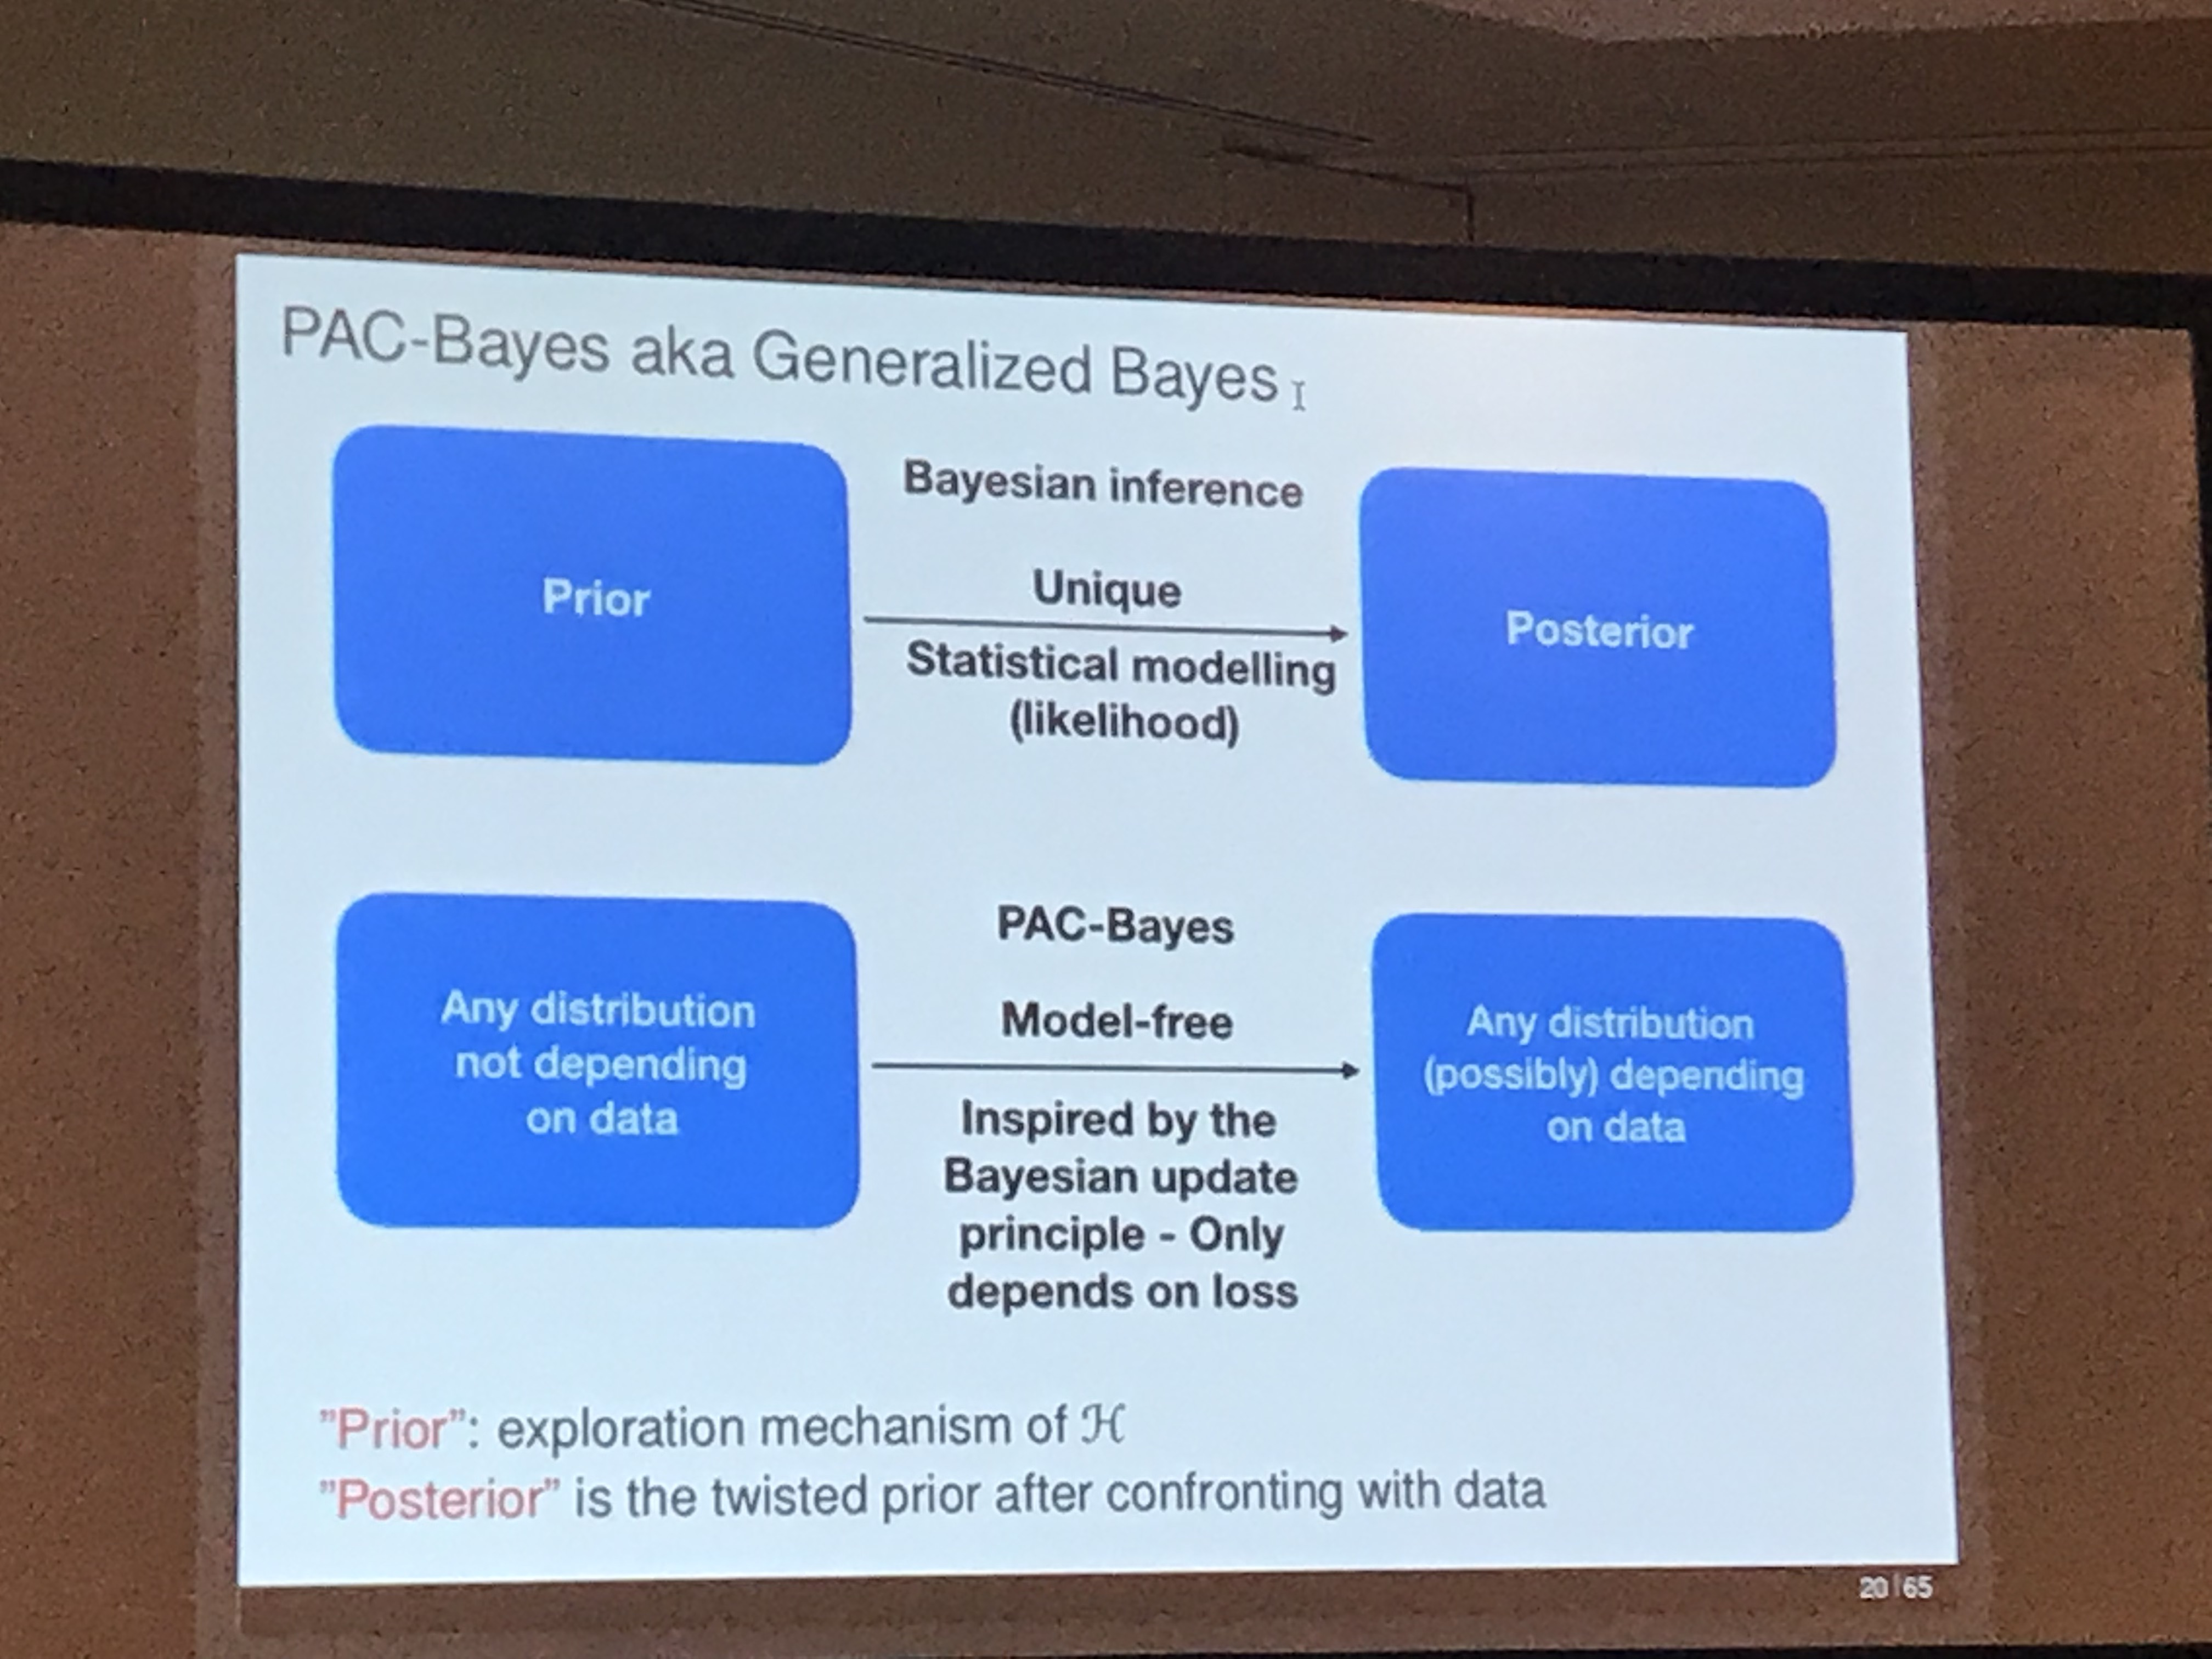
\includegraphics[width=0.5\textwidth]{images/pb1.JPG}
    \caption{Differences in Bayes and PAC-Bayes}
    \label{fig:pac_bayes}
\end{figure}


\begin{theorem}
\label{thm:pac_bayes}
(\citet{mcallester1999some}) For any prior $P$, $\delta \in (0,1]$, we have:
\begin{equation}
    \Pr\left(\forall_{Q \in \mc{H}} : R_{out}(Q) \leq R_{in}(Q) + \sqrt{\frac{\KL{Q}{P}) + \ln \frac{2 \sqrt{m}}{\delta}}{2m}}\right) \geq 1-\delta,
    \label{eq:pac_bayes}
\end{equation}
where $\mc{H}$ is the hypothesis space, $m$ is the number of samples, $R_{out}$ is the risk of a hypothesis on the test data, $R_{in}(h)$ is the risk of the data on the training data, $P$ is the prior, and $Q$ is the posterior.
\end{theorem}

PAC-Bayes: a flexible learning theoretic framework! Tight connections to regression, linear classification \& SVMs, transductive learning, uses in RL~\cite{fard2010pac}, and more.


\subsubsection{PAC-Bayes Theory}
This section explores the high level view of PAC-Bayesian Theory. \\

Q: How can PAC-Bayes drive learning? \\

A: First, recall:
\begin{equation}
    R_{out}(Q) \leq R_{in}(Q) + F(Q),
\end{equation}
Or:
\begin{equation}
    \text{Error on unseen data} \leq \text{Error on sample + complexity term}.
\end{equation}

This definse a [rinciple strategy for obtaining new algorithms:
\begin{align}
    &h \sim Q^* \\
    &Q^* \in \text{arginf}_{Q \ll P} \left\{R_{in}(Q) + F(Q)\right\}.
\end{align}

Presents an optimization problem: can be solved or approximated to find good solutions! \\

PAC-Bayes interpretation of celebrated algorithms: 
\begin{itemize}
    \item SVM with a sigmoid loss and KL-regularized Adaboost canm be reinterpreted as minimizer of PAC-Bayesian bounds~\cite{ambroladze2007tighter}.
    \item Also, the minimizer of:
    \[
    \left\{R_{in}(Q) + \frac{KL}{\lambda}\right\},
    \]
    is the celbrated Gibbs posterior:
    \[
    Q_\lambda(h) \propto \exp(-\lambda R_{in}(h)) P9h), \hspace{5mm} \forall_{h \in \mc{H}}.
    \]
    
    When $\lambda \ra 0$, we get a flat posterior, and as $\lambda \ra \infty$, we get Dirac mass on expected risk minimization (ERMs).
\end{itemize}



\begin{theorem}
\[
\log \int (\exp \phi) dP = \sup_{Q \ll P} \left\{ \int \phi dQ - KL(Q,P)\right\}.
\]
\end{theorem}
\begin{proof}
First require variational definition of KL-Divergence~\cite{csiszar1975divergence}
\begin{align}
    -\KL{Q}{G} &= - \int \log\left(\frac{dQ}{dP} \frac{dP}{dG}\right) dQ \\
    &= -\KL{Q}{P} + \int \phi dp - \log \int(\exp \phi) dP.
\end{align}
Note that KL is non negative, $Q \ra -\KL{Q}{P}$ reaches its max in $Q=G$. Thus, taking $\phi = -\lambda R_{in}$:
\[
Q_\lambda(h) \propto \exp(-\lambda R_{in}(h)) P9h), \hspace{5mm} \forall_{h \in \mc{H}}. \qedhere
\]
\end{proof}

Q: What about non-i.i.d. data? \\

A: Sure! Let's drop the i.i.d. and bounded loss assumptions. First, consider the moment of a distribution:
\ddef{Moment}{The $p$-th moment of a distribution is given by:
\[
M_p := \int \bE\left[|R_{in}(h) - R_{out}(h)|^p )\right) dP(h).
\]}

Also make use of $f$-divergences, a generalization of the KL-Divergence. \\

\begin{theorem}
Let $\phi_p : x \mapsto x^p$. Fix $p > 1, q = \frac{p}{p-1}$ and $\delta \in (0,1)$. W/ probability at least $1-\delta$, for any distr. $Q$:
\[
|R_{out}(Q) - R_{in}(Q)| \leq (\frac{M_q}{\delta}^{1/q}(D_{\phi_{p-1}}(Q,P) + 1)^{1/p}.
\]
\end{theorem}

Takeaway: we can bound generalization error using the $f$-divergence ($D_{\phi_{p-1}}$ and moment $(M_q)$. Proof strategy requires: 1) Jensen's inequality, 2) change of measure, 3) Holder's inequality, and 4) Markov's inequality. \\

Oracle Bounds;~\citet{catoni2007pac} derived PAC-Bayesian bounds for the Gibbs posterior.

\subsubsection{PAC-Bayes and Task Awareness}

Note: PAC-Bayesian bounds express a tradeoff between empirical accuracy and a measure of complexity. \\

Q: So, how can we improve the bounds we get? How do we choose the right prior distribution so that we can 1) control complexity, and 2) ensure good performance? \\

$\ra$ So: can we choose a ``better' prior? (without looking at the test data itself?) \\

{\bf Main Idea:} use part of the data to learn how to choose a prior. \\

Can use PAC-Bayes in SVMs:
\begin{itemize}
    \item Assume prior and poster are spherical Gaussians (w/ prior centered at origin, posterirer centered at a scaling $\mu$ of unit SVM weight vector).
    \item Implies that KL term in generalization error bound is $\mu^2 / 2$ (see Theorem~\ref{thm:pac_bayes}).
    \item Can computer schochastic error of posterior distribution behaves like a soft margin, scaling $\mu$ trades between margin loss and KL.
    \item Bound holds for all $\mu$, so choose $\mu$ to optimize the bound.
\end{itemize}

Q: But how do we learn the prior for SVMs?
\begin{itemize}
    \item Bound depends on distance between prior and posterir
    \item Better prior means tighter bound
    \item Idea: learn prior $P$ with part of the data.
    \item Introduce learnt prior in the bound.
    \item Computer stochastic error with remaining data: PrPAC.
    \item Can go a step further: 1) scaling the prior in the chosen direction $\tau$-PrPAC, or 2) Adapt SVM to optimize the new bound: $\eta-$Prior SVM.
\end{itemize}

Results from the above methods for tightening the bounds: see Figure~\ref{fig:pb_results}. \\

\begin{figure}
    \centering
    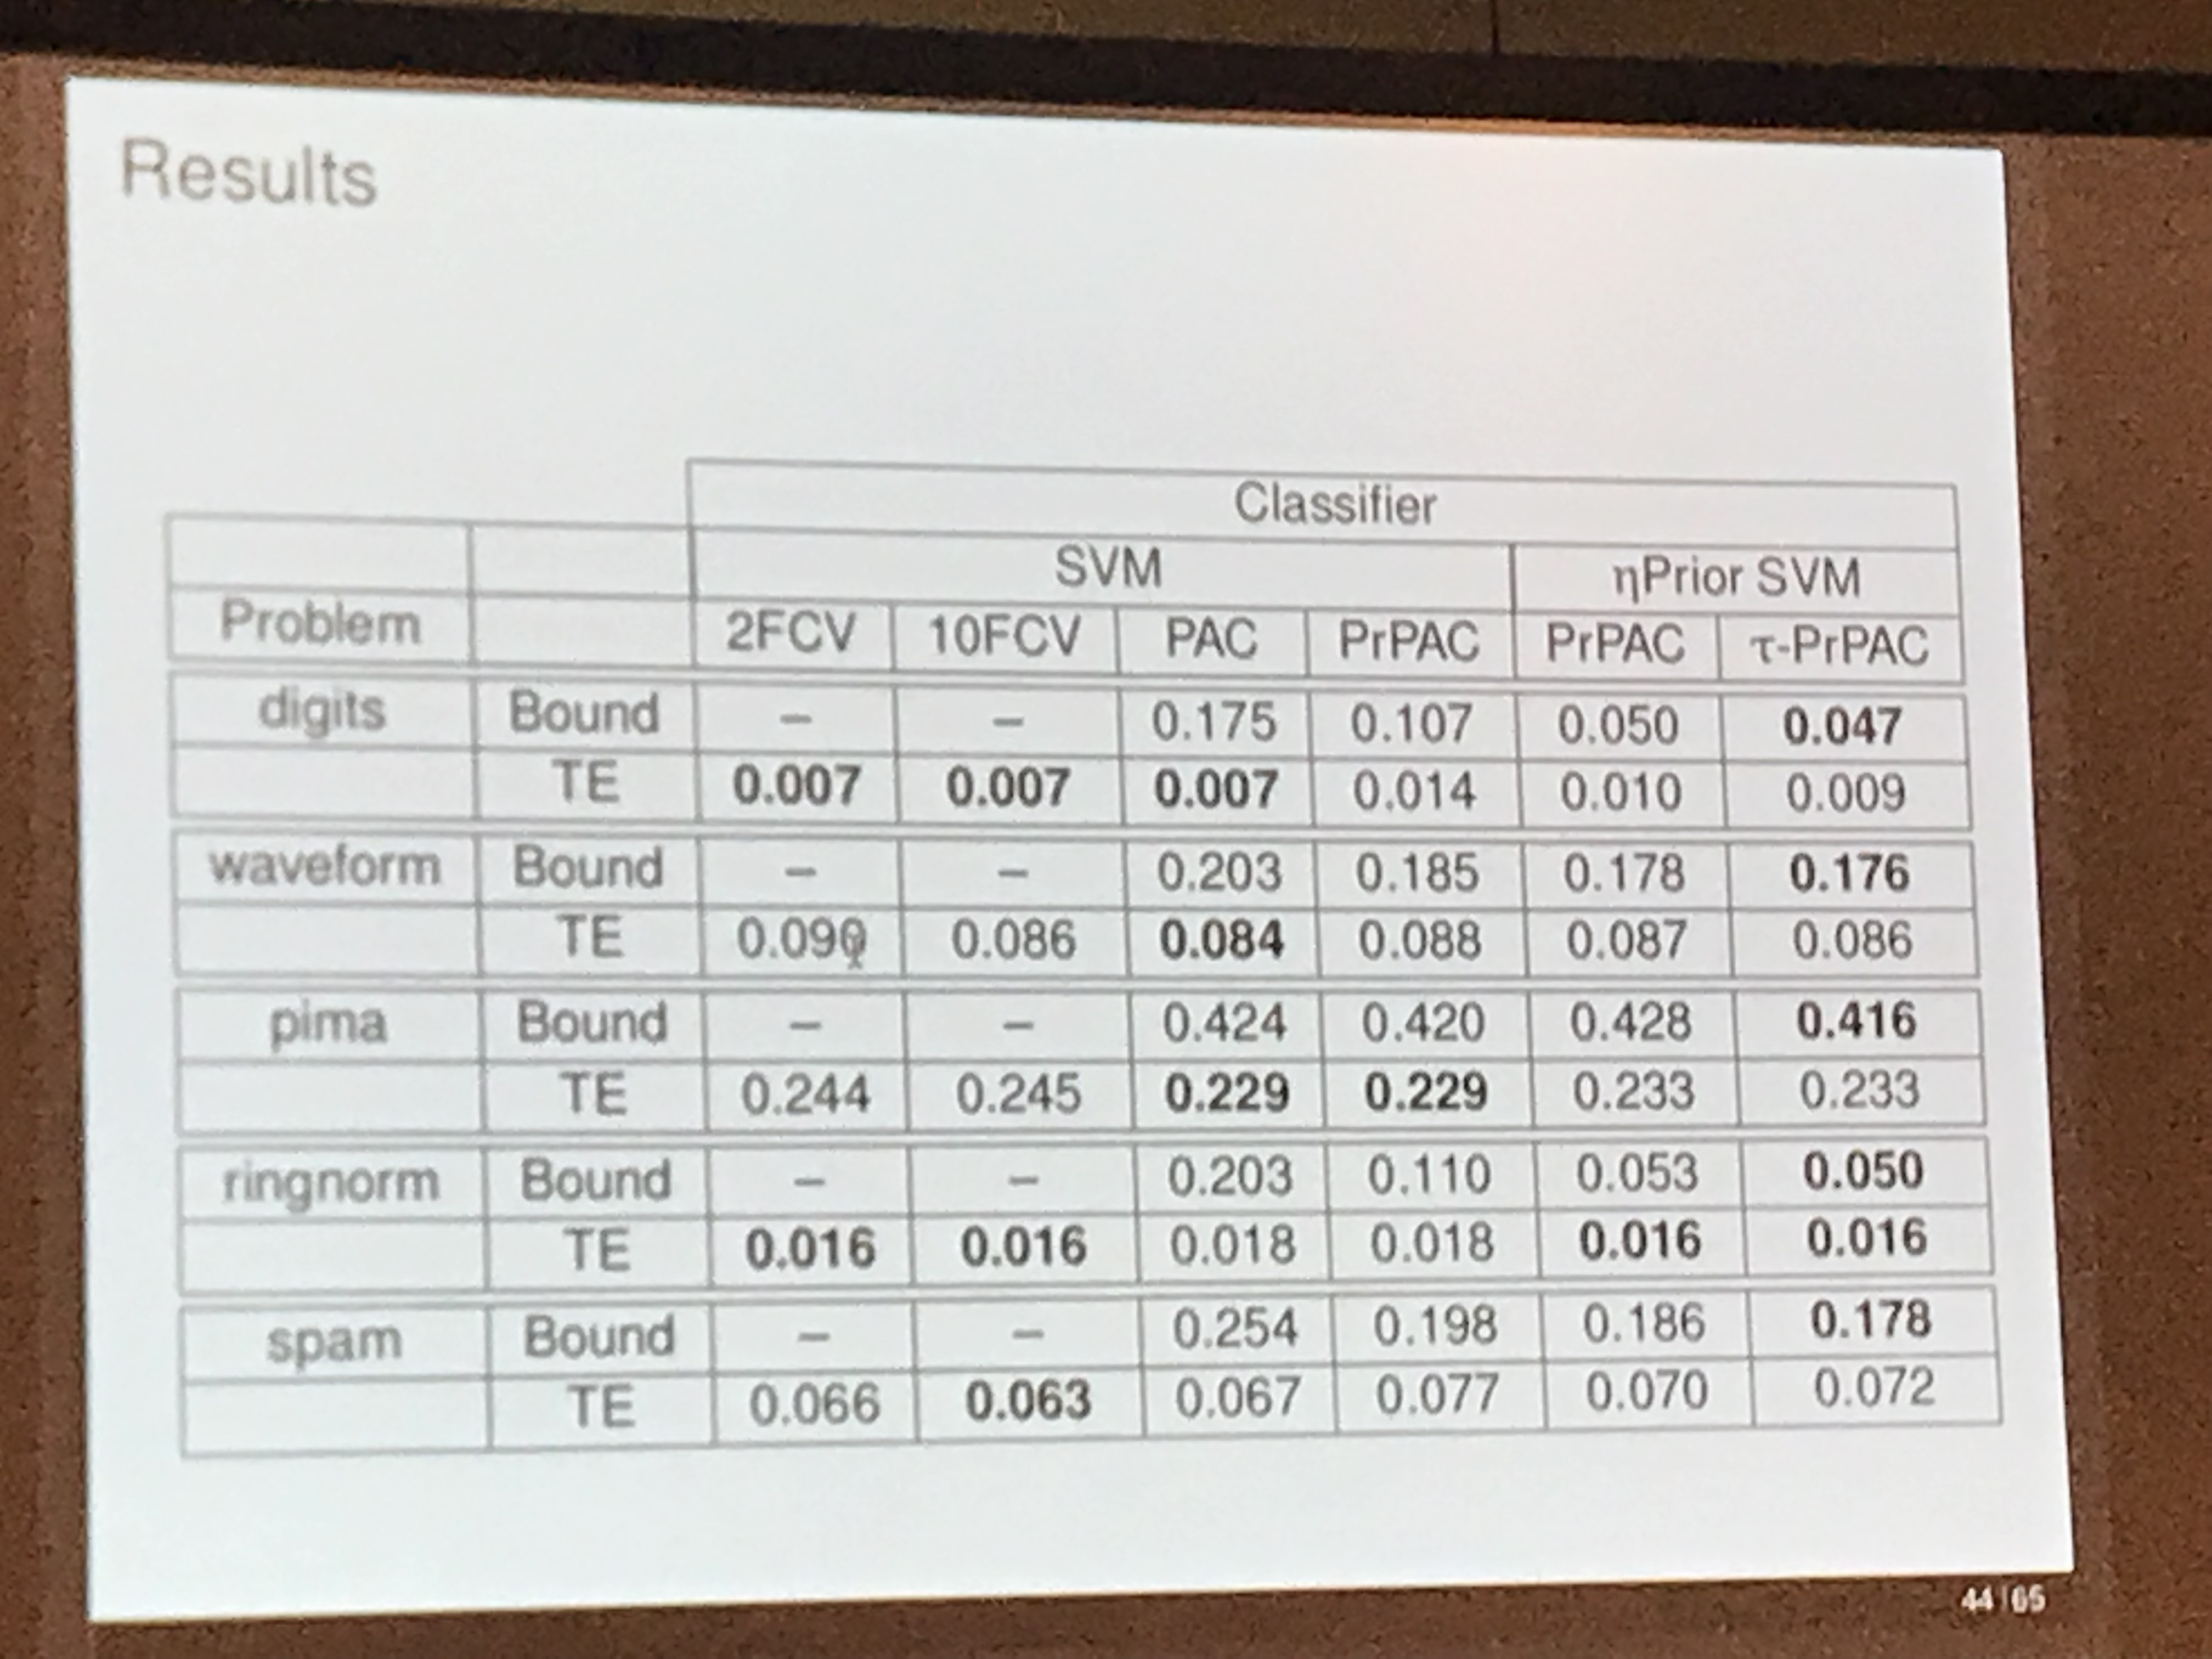
\includegraphics[width=0.5\textwidth]{images/pb_results.JPG}
    \caption{Results from applyinh differnet PAC-Bayes prior selection methods to experiments.}
    \label{fig:pb_results}
\end{figure}

Takeaways from results:
\begin{enumerate}
    \item Bounds are remarkably tight!
    \item Model-selection via these new bounds is {\it as good} as 10-fold cross validation.
    \item Best bounds don't necessarily translate into best model selection.
    
    $\ra$ We're not {\it completely} capturing the right thing (but definitely some of the right thing).
\end{enumerate}

Next up: distribution-defined priors:
\begin{itemize}
    \item Consider $P$ and $Q$ are Gibbs-Boltzmann distributions:
    \[
    P_\gamma(h) = \frac{1}{Z} \exp(-\gamma R_{out}(h) \hspace{8mm} Q_\gamma(h) = \frac{1}{Z}\exp(-\gamma R_{in}(h)).
    \]
    \item These distributions hard to work with since we can't apply it to a single weight vector. From~\citet{catoni2007pac}, we can show:
    \[
    \KL{R_{in}(Q_\lambda)}{R_{out}(Q_\lambda)} \tilde{\leq} \frac{1}{m} \left(\gamma / \sqrt{m} + \gamma^2/4m\right),
    \]
    where $\tilde{\leq}$ ignores log terms on the right hand side (\dnote{my (awful) construction for abbreviation, not theirs}).
    
\end{itemize}

On stability:
\begin{itemize}
    \item If $A$ has sensisitivty $\beta$ at sample size $m$, then generalization error can be bounded~\cite{bousquet2002stability}.
    
    \item Q: Algorithm output is highly concentrated, does that imply stronger results?
    
    $\ra$ Yes! We can derive (tighter) bounds that depend on KL between a distributionally sensitive prior and a well chosen posterior.
    
    Open area! Lots of room to explore a new kind of generalization error analysis.
\end{itemize}

{\bf A final case study:} Can we use any of this to analyze deep neural networks? \\

Q: Is deep learning breaking the statistical paradigm we know? \\

$\ra$ Neural nets trained on massive datasets achieve {\it zero training error}, which does not bode well for their performance. Yet! They tend to achieve remarkably low error on test sets, too. \\

{\bf Idea:} Perhaps we can use PAC-Bayes to explain this phenomena. \\



\begin{figure}
    \centering
    \subfloat[Classical view of Overfitting]{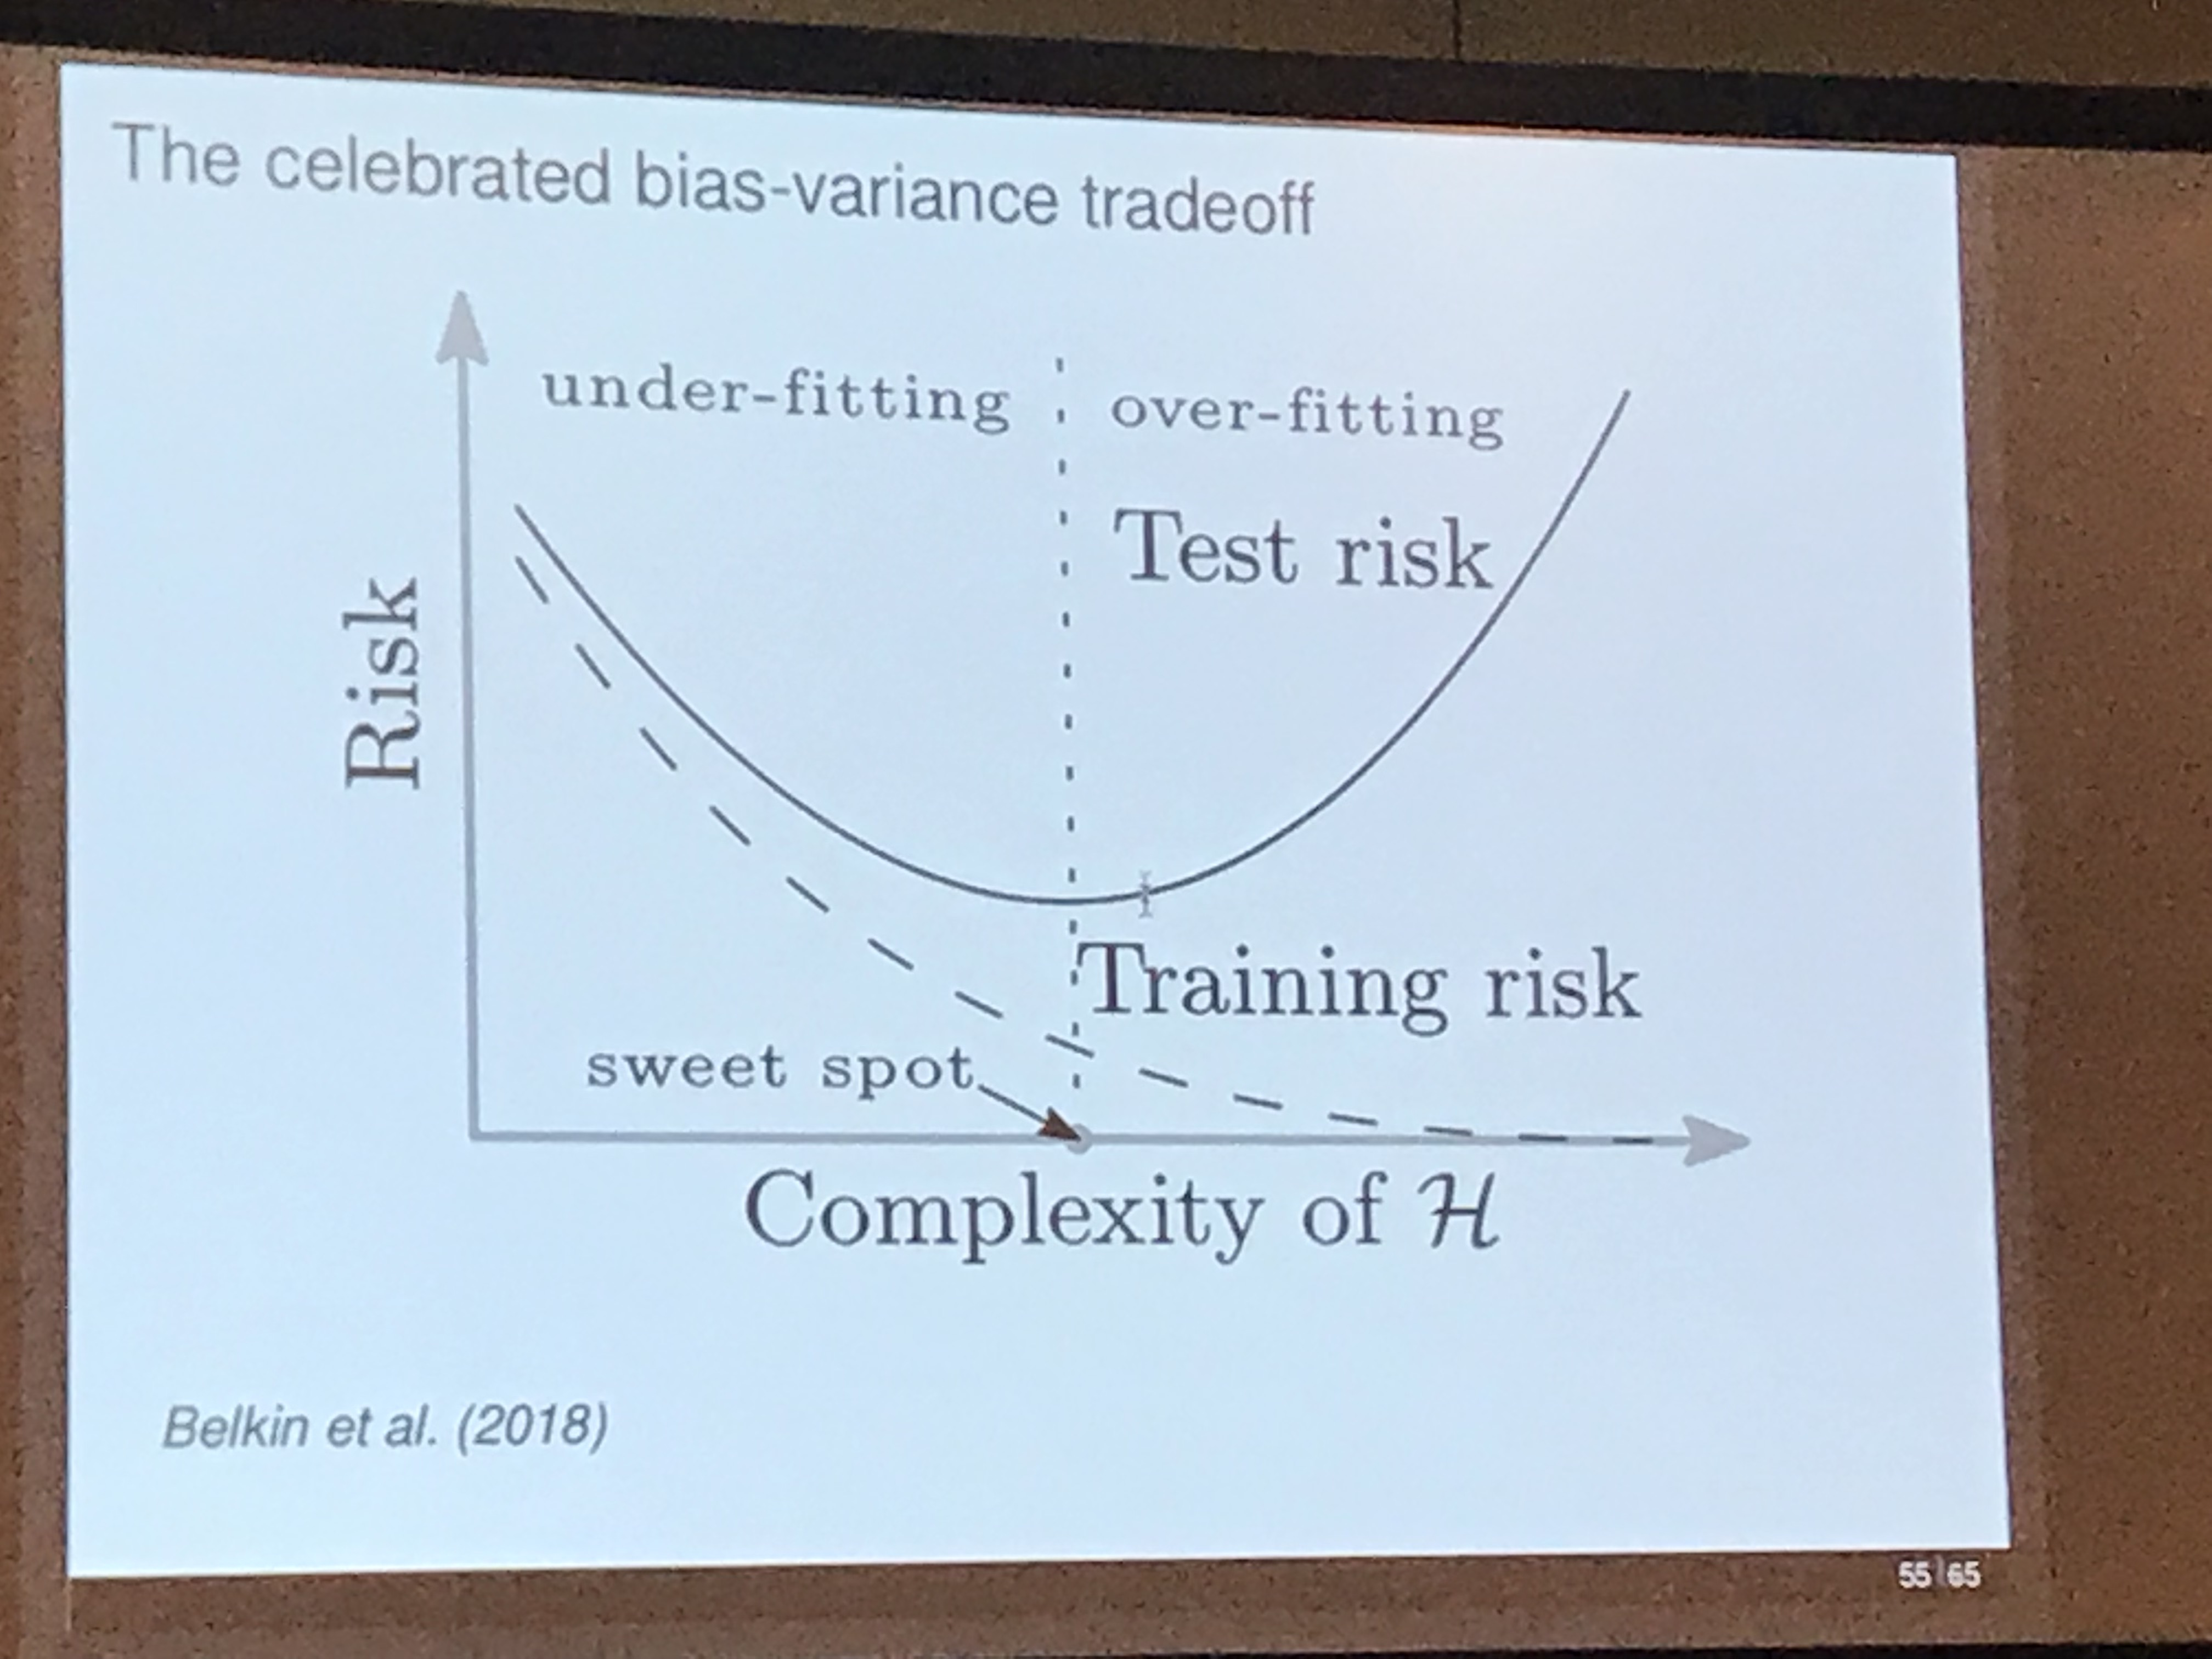
\includegraphics{images/of.JPG}}
    \subfloat[New Paradigm?]{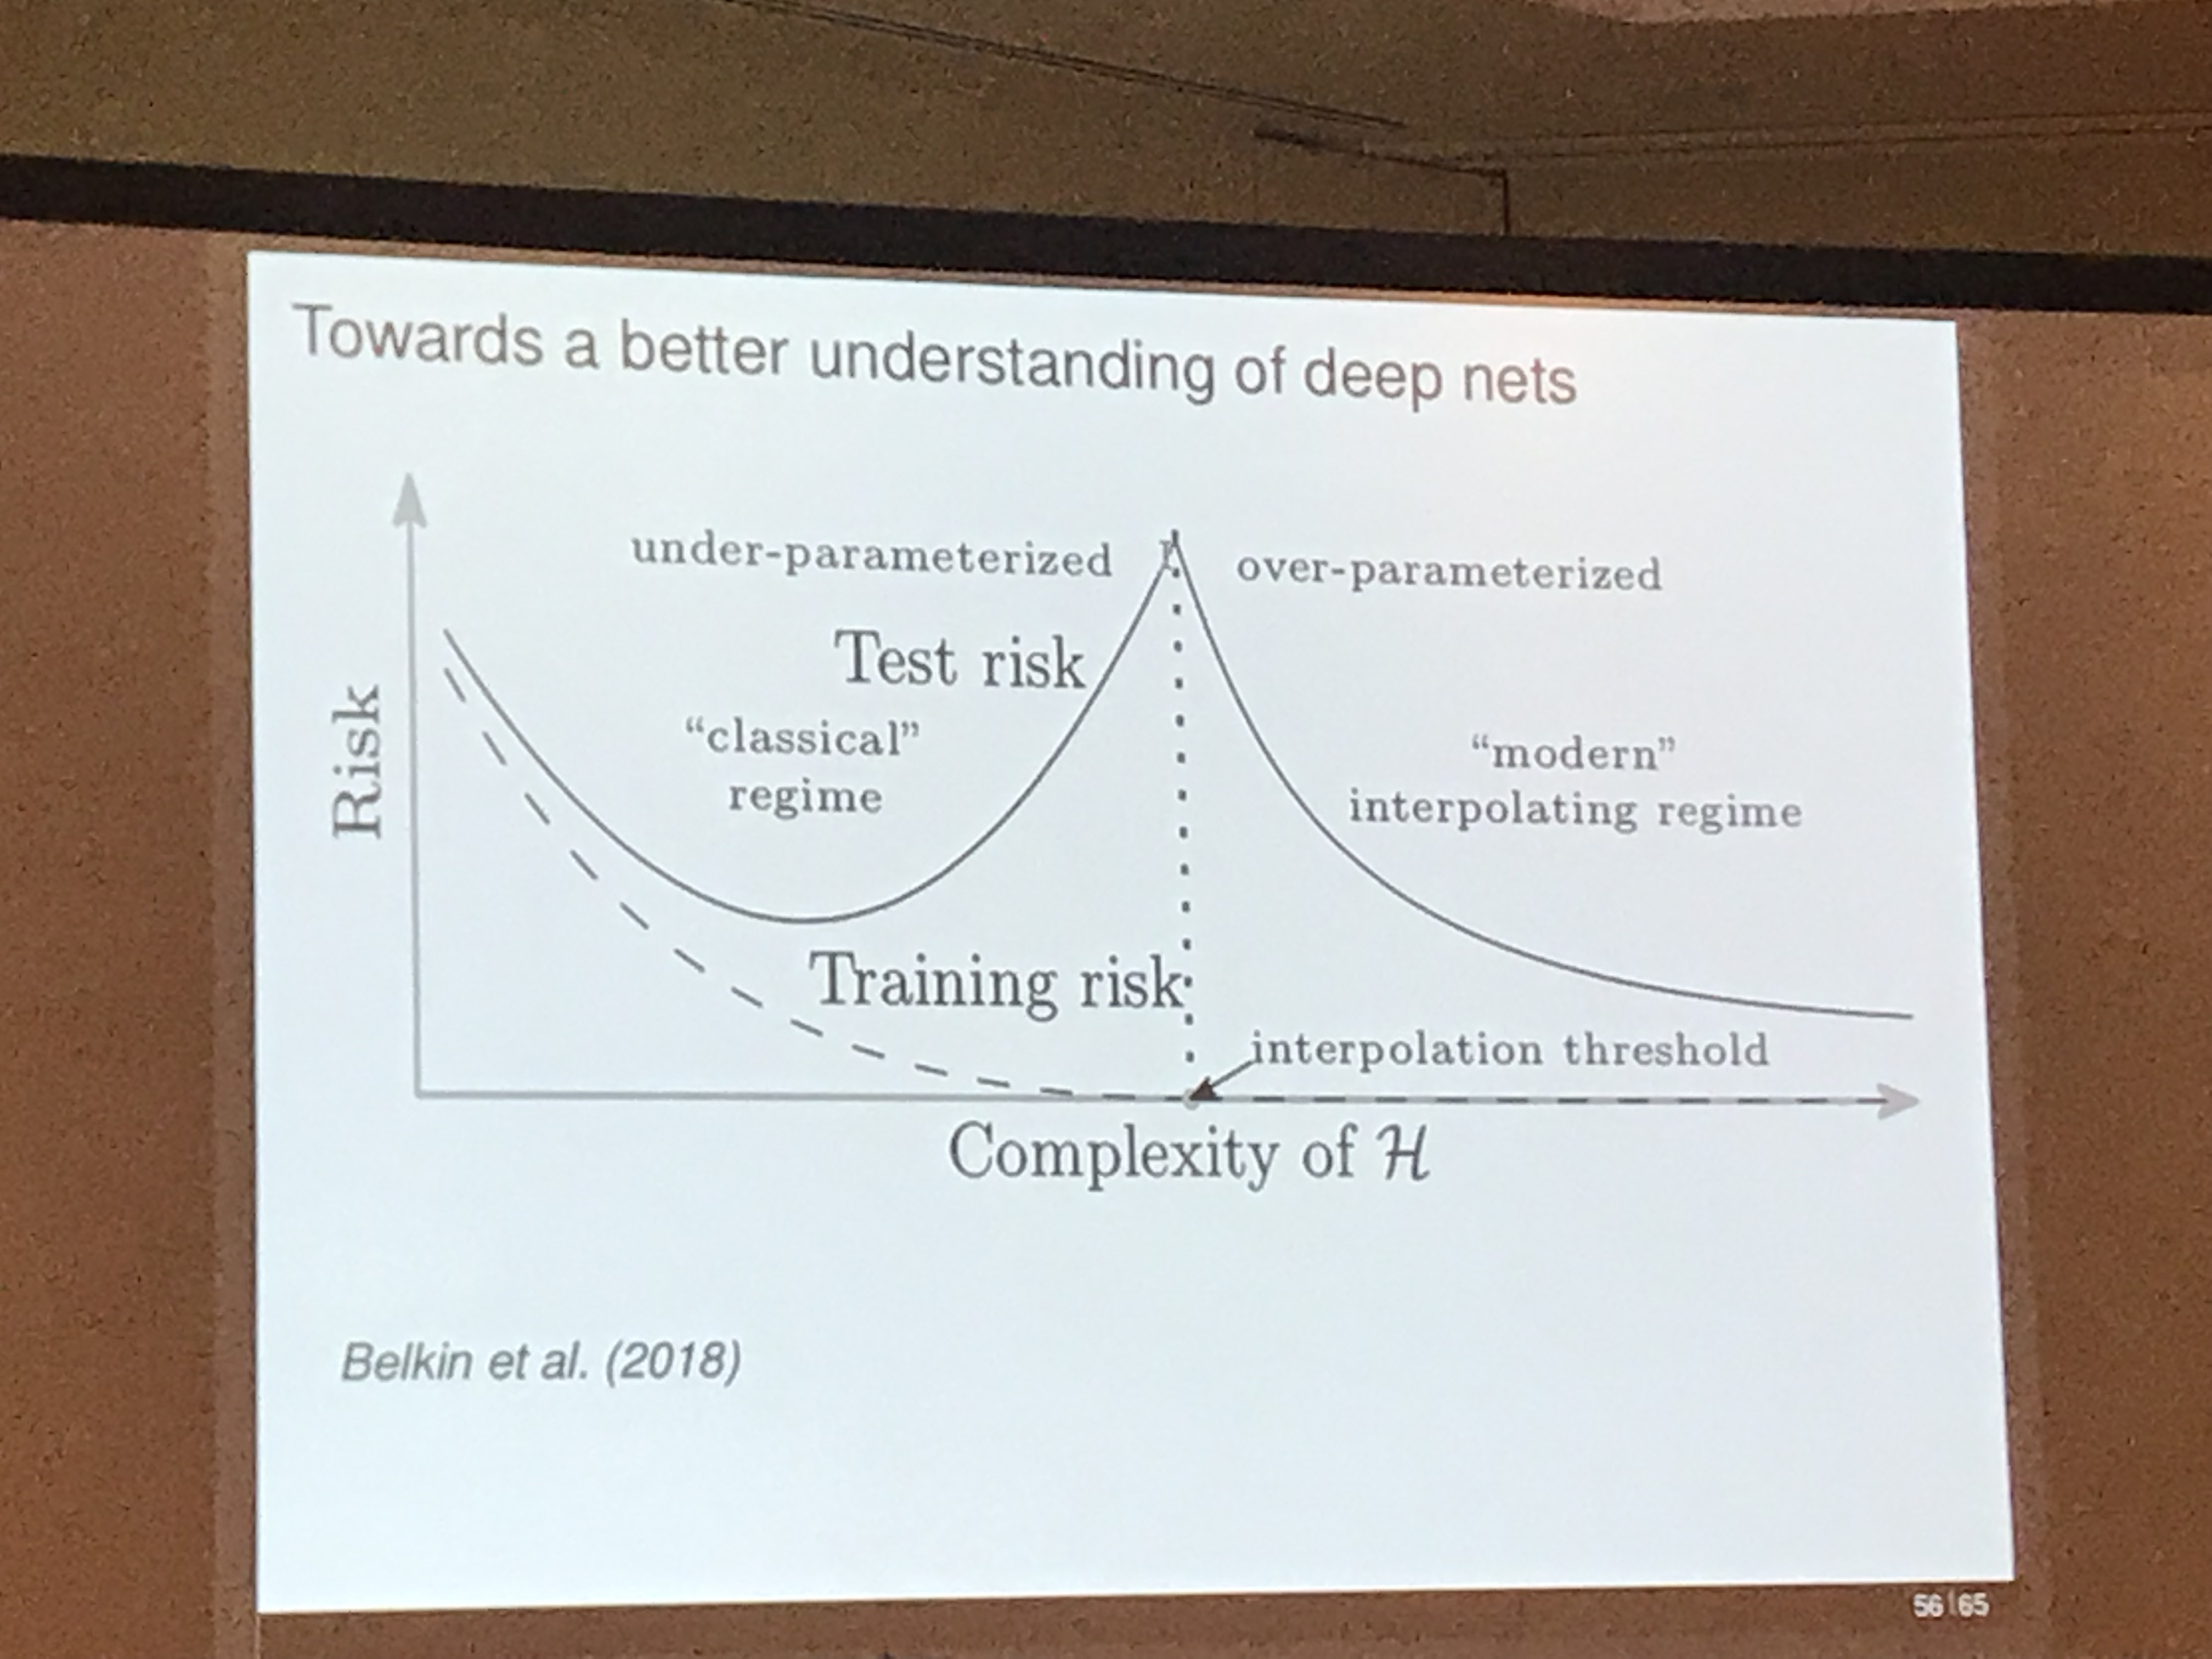
\includegraphics{images/of_2.JPG}}
    \caption{Classical view of overfitting (left), and a new proposal for why deep nets might be avoiding overfitting (right), from~\citet{belkin2018overfitting}.}
    \label{fig:overfitting}
\end{figure}

~\citet{dziugaite2017entropy} derived extremely tight deep learning generalization error bounds in this way;
\begin{itemize}
    \item Based on training to expand the ``basin of attraction"
    \item Hence, not measuring good generalization of {\it normal training}
\end{itemize}

Q: How much information is contained in the training set? \\

A1: ~\citet{achille2018information} studied the {\it amount of information} stored in the weights of deep networks. Overfitting might be related to information being stored in weights that encode training set, as opposed to the data generation distribution. \\

A2: Information bottleneck criterion~\cite{} might control this information, and could lead to a tighter PAC-Bayes bound. \\

{\bf Conclusions:}
\begin{itemize}
    \item PAC-Bayes arises from two fields: 1) statistical learning theory, and 2) Bayesian Learning
    \item Generlazies both fields and points to promising directions
    \item PAC-Bayes theory can be an inspiration toward new theoretical analysis, but also drive algorithm design (especially when theory has proven difficult).
\end{itemize}